\section{\Glsfmtlong{cml-glossary} Experiment Implementation}

The current state of the art for median filtering is quite sophisticated, and algorithms have been developed that are very fast \cite{Sanchez2012,Perrot2014} or can significantly restore an image even at a noise level of over 90\% \cite{Gao2015,Wu2011}.  Such algorithms were not used here because the focus was on comparing the performance of some relatively straightforward implementations.

An implementation of the basic \gls{medianfilter} was created in \fsharp{}, using the \hopac{}\footnote{\url{https://github.com/hopac/hopac}} \gls{cml} library.  For comparison, two other parallel implementations were created in \fsharp{}, one a naïve implementation that simply uses nested \texttt{for loop}s to operate over the relevant window, and another loosely based on the \gls{medianfilter} algorithm described by \citeauthor{Braunl2001} \cite{Braunl2001}.\footnote{All three implementations, as well as other relevant files and benchmarking results, are available at \url{https://github.com/jcoo092/ivcnz2018}}

\fsharp{} was chosen because of the easy availability of a ready-to-use \gls{cml} library, as well as its relative similarity to the original Standard ML host language.  Of particular note is that the original \gls{cml} implementation assumed the presence of garbage collection, which Hopac also follows.  Faster versions of the other algorithm variants likely could have been implemented in other languages such as C/C++ (perhaps using Halide \cite{Ragan-Kelley2017}), Fortran or Rust, but \fsharp{} was used for all three to retain consistency and comparability.  

All three algorithms were benchmarked using a variety of image and window sizes.  Window sizes of 3×3, 5×5, 7×7, 9×9 and 11×11 were measured.  The images used ranged in size from 15 kilopixels to 1.09 megapixels, as detailed in \Cref{tab:median:pixelcounts}.  Larger image sizes were initially attempted, but some runs of the algorithms proved to be prohibitively slow, and so they were abandoned.  Time spent on loading the images from disk and converting them to greyscale was excluded from the benchmarking, so that only the time spent processing them with each algorithm was measured.  The benchmarks were all run using .NET Core 2.1.4 with the 64-bit RyuJit compiler, on a desktop computer with a quad-core Intel i7-7700 processor running at 3.6GHz and 16GB of RAM.

\begin{table}
\centering
\caption{List of pixel counts for each image used}
\label{tab:median:pixelcounts}
\begin{tabular}{@{}lccc@{}}
\toprule
\textbf{Image} & \multicolumn{1}{c}{\textbf{Width (px)}} & \multicolumn{1}{c}{\textbf{Height (px)}} & \multicolumn{1}{c}{\textbf{Total pixels (px)}} \\ \midrule
very small                         & 150                                     & 100                                      & 15,000                                         \\
peppers                            & 512                                     & 512                                      & 262,144                                        \\
small                              & 640                                     & 426                                      & 272,640                                        \\
medium                             & 1280                                    & 853                                      & 1,091,840                                      \\ \bottomrule
\end{tabular}
\end{table}

\subsection{Operation of algorithms}
The naïve algorithm used a simple nested \texttt{for loop} approach.  For every pixel in the image, an array was declared with length equal to the total size of the window, and then nested \texttt{for loop}s spanning that size were used to iterate over the pixels in the window and collect their intensity values into the array.  Each array was then processed to determine the median, with the result returned as the value for that pixel in the new image.

The Bräunl-inspired algorithm used here does not precisely match that of \cite{Braunl2001}, primarily because it was unclear how boundary conditions were handled there, but also because the book's algorithm assumed a 3×3 window.  It sits roughly between the other two approaches, in that it simply reads the value of neighbouring horizontal pixels from an array then sends that list to its vertical neighbours to combine and find the median.  This functionality was replicated in the implementation insofar as possible, but the book's algorithm assumes the use of the domain-specific language Parallax, which automatically operates on whole images.

The \gls{cml} algorithm transforms each pixel into a logical \glsxtrlong{pe} (essentially the \glspl{pe} of \cref{chap:nmp}) with a channel, on which it always offers to give its intensity value, and a reducing list of its neighbours, to which it offers to take their intensity value.\footnote{By default, \gls{cml} does not provide facilities for antiport-style messaging, necessitating this approach instead.}  Once all neighbouring values have been taken, they are combined and the median found and stored in the output array.  The pixel then enters a loop (implemented as a tail-recursive function, in traditional \gls{cml} style) whereby it always offers to give its intensity value via its channel.  This is required to ensure that any subsequent requests from other pixels to take the intensity from that pixel can be fulfilled.

Boundary conditions in all three cases were handled by utilising the \texttt{Option}\footnote{See \url{https://docs.microsoft.com/en-us/dotnet/fsharp/language-reference/options} for a brief overview on \texttt{Option} types, or \eg{} \cite{Syme2015a} for a more comprehensive explanation.} type in \fsharp{}, where \texttt{None}s were returned for pixels outside the images, which were filtered out after the complete window had been collected, and the median selected from those remaining.  The same process was used for determining the median in the returned array across the algorithms.  An in-place sort function was called on the array, and then the element at the position \(\mathit{length} \div 2\) was returned.

It should be noted that in all three instances the specifics of parallelising the execution of the tasks is left up to the .NET or \hopac{} runtimes.  No explicit creation, management or scheduling of threads is performed in the written programs.  Instead, the programs explore different approaches to structuring the computation in code.

\section{Results}

\Crefrange{tab:median:verysmall}{tab:median:medium} show the mean of the benchmarking results of running each algorithm on each of the different images, across the window sizes.  \Crefrange{graph:median:verysmall}{graph:median:medium} are charts visualising the results in the tables.  \Cref{graph:median:cmls} plots the mean runtimes for the \gls{cml} algorithm at each window size for each image.  All the charts use a y axis with a logarithmic scale because it makes a visual comparison easier here.

The naïve algorithm performs the best for every image and window size, while the Bräunl algorithm matches it reasonably closely, though always running a bit more slowly.  Both appear to scale moderately well, roughly doubling in runtime for every increase by 2 of the size of a side of the window, whereas the \gls{cml} algorithm appears to follow an exponential increase in runtime.  The reason for this is not certain, but it appears that the \gls{cml} approach creates considerable pressure on the memory heap, causing numerous expensive garbage collections.  These collections do have the benefit of keeping the peak memory consumption relatively low, however.

The ratios of the runtimes of the Bräunl and \gls{cml} algorithms compared to the runtime for the naïve algorithm for each image and window size are presented in \cref{tab:median:ratbraun,tab:median:ratcml}.  While the ratios for the Bräunl algorithm worsen for increasing image sizes, they, in fact, improve for larger window sizes on the same image, suggesting that it scales better than the naïve in this regard.  Why that should be is unclear.  No pattern can be discerned for the \gls{cml} algorithm, however, besides that the ratio for the same window size typically grows worse as image size increases.

To provide a rough estimate of the effects of the median filtering, a copy of each base image was created with randomly introduced salt \& pepper noise.  \Cref{fig:median:peppers} shows the outputs for the peppers image using a window size of 3, along with the base and noisy images.  None of the algorithms restored the original image perfectly, but all have largely eliminated the noise, at the cost of a slight blurring.  The results for each were measured using the classic peak signal-to-noise ratio formula \cite{Boncelet2005}, and are presented in \crefrange{tab:median:psnrvsmall}{tab:median:psnrmedium}.  The naïve and \gls{cml} algorithms return near-identical results, while Bräunl always falls somewhat short.

\begin{table}
\centering
\caption[Mean runtimes for each algorithm for the `very small' image]{Mean runtimes for each algorithm by window size for the `very small' image}
\label{tab:median:verysmall}
\begin{tabular}{@{}lrrrrr@{}}
\toprule
\multicolumn{1}{c}{\textbf{Algorithm}} & \multicolumn{5}{c}{\textbf{Mean time for each window size (ms)}} \\
                              & 3        & 5         & 7         & 9         & 11       \\ \midrule
Naïve                         & 1.623    & 3.983     & 7.578     & 12.483    & 18.933   \\
Bräunl                        & 5.462    & 10.195    & 15.973    & 22.807    & 31.843   \\
\gls{cml}                           & 50.588   & 118.463   & 212.817   & 299.339   & 510.526  \\ \bottomrule
\end{tabular}
\end{table}

\begin{table}
\centering
\caption[Mean runtimes for each algorithm for the `peppers' image]{
\label{tab:median:peppers}Mean runtimes for each algorithm by window size for the `peppers' image}
\begin{tabular}{@{}lrrrrr@{}}
\toprule
\multicolumn{1}{c}{\textbf{Algorithm}} & \multicolumn{5}{c}{\textbf{Mean time for each window size (ms)}}  \\
                              & 3       & 5         & 7         & 9         & 11         \\ \midrule
Naïve                         & 36.474  & 77.122    & 144.854   & 232.750   & 371.789    \\
Bräunl                        & 108.436 & 206.336   & 296.717   & 463.857   & 592.056    \\
\gls{cml}                           & 791.285 & 2,333.317 & 4,452.903 & 7,533.048 & 11,237.458 \\ \bottomrule
\end{tabular}
\end{table}

\begin{table}
\centering
\caption[Mean runtimes for each algorithm for the `small' image]{Mean runtimes for each algorithm by window size for the `small' image}
\label{tab:median:small}
\begin{tabular}{@{}lrrrrr@{}}
\toprule
\multicolumn{1}{c}{\textbf{Algorithm}} & \multicolumn{5}{c}{\textbf{Mean time for each window size (ms)}}  \\
                              & 3       & 5         & 7         & 9         & 11         \\ \midrule
Naïve                         & 35.246  & 75.282    & 141.432   & 231.667   & 343.286    \\
Bräunl                        & 116.782 & 215.573   & 313.114   & 472.517   & 629.898    \\
\gls{cml}                           & 849.482 & 2,362.643 & 4,830.294 & 7,910.925 & 12,074.170 \\ \bottomrule
\end{tabular}
\end{table}

\begin{table}
\centering
\caption[Mean runtimes for each algorithm for the `medium' image]{Mean runtimes for each algorithm by window size for the `medium' image}
\label{tab:median:medium}
\begin{tabular}{@{}lrrrrr@{}}
\toprule
\multicolumn{1}{c}{\textbf{Algorithm}} & \multicolumn{5}{c}{\textbf{Mean time for each window size (ms)}}      \\
\multicolumn{1}{r}{}                   & \multicolumn{1}{r}{3} & 5         & 7         & 9         & 11        \\ \midrule
Naïve                                  & 131.111               & 288.343   & 549.600   & 899.563   & 1,361.629 \\
Bräunl                                 & 589.431
               & 899.233   & 1,433.22  & 1,933.76  & 2,447.28  \\
\gls{cml}                                    & 4527.962
               & 11,006.78 & 21,210.30 & 34,587.35 & 56,196.61 \\ \bottomrule
\end{tabular}
\end{table}

\begin{table}
\centering
\caption[Ratios runtime for the Bräunl algorithm vs the naïve algorithm]{Ratios of length of runtime for the Bräunl algorithm compared to the naïve algorithm for the same image and window sizes}
\label{tab:median:ratbraun}
\begin{tabular}{@{}lccccc@{}}
\toprule
\textbf{Image} & \multicolumn{5}{c}{\textbf{Window Size}} \\
               & 3      & 5      & 7      & 9     & 11    \\ \midrule
very small     & 3.37   & 2.56   & 2.11   & 1.83  & 1.68  \\
peppers        & 2.98   & 2.68   & 2.05   & 2.00     & 1.62  \\
small          & 3.32   & 2.86   & 2.21   & 2.04  & 1.83  \\
medium         & 4.51   & 3.12   & 2.61   & 2.15  & 1.80   \\ \bottomrule
\end{tabular}
\end{table}

\begin{table}
\centering
\caption[Ratios of runtime for the \glsentrylong{cml-glossary} algorithm compared to the naïve algorithm]{Ratios of length of runtime for the \gls{cml} algorithm compared to the naïve algorithm for the same image and window sizes}
\label{tab:median:ratcml}
\begin{tabular}{@{}lccccc@{}}
\toprule
\textbf{Image} & \multicolumn{5}{c}{\textbf{Window Size}} \\
               & 3      & 5      & 7      & 9     & 11    \\ \midrule
very small     & 31.18  & 29.75  & 28.08  & 23.98 & 26.97 \\
peppers        & 21.73  & 30.29  & 30.83  & 32.49 & 30.74 \\
small          & 24.12  & 31.39  & 34.15  & 34.15 & 35.17 \\
medium         & 34.65  & 38.19  & 38.61  & 38.45 & 41.29 \\ \bottomrule
\end{tabular}
\end{table}

%very small
\begin{figure}
\centering
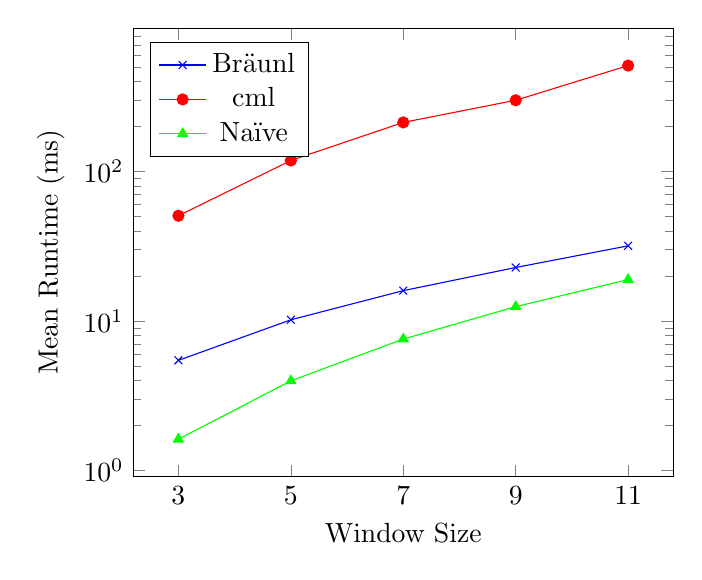
\begin{tikzpicture}
\begin{semilogyaxis}[
	xlabel=Window Size,
    ylabel=Mean Runtime (ms),
    legend pos=north west,
    %xmin=3,
    %xmax=11,
    %minor x tick num=2,
    xtick=data
]
	\addplot [mark=x,blue] table [x=windowSize,y=Mean]{
    	Method	windowSize	filename	Mean	Error	StdDev	Median	Min	Scaled	ScaledSD	Gen0	Gen1	Gen2	Allocated
Bräunl	3	very-small	5.462	0.109	0.285	5.461	4.696	3.37	0.17	31.25	15.625	15.625	2.11
Bräunl	5	very-small	10.195	0.202	0.543	10.087	9.467	2.56	0.14	46.875	31.25	15.625	3.52
Bräunl	7	very-small	15.973	0.318	0.724	15.830	15.012	2.11	0.09	46.875	15.625	-	6.04
Bräunl	9	very-small	22.807	0.447	0.829	22.497	21.855	1.83	0.07	93.75	31.25	-	9.86
Bräunl	11	very-small	31.843	0.621	0.891	31.955	29.750	1.68	0.05	187.5	62.5	-	15.63


    };
    \addplot [mark=*,red] table [x=windowSize,y=Mean]{
    	Method	windowSize	filename	Mean	Error	StdDev	Median	Min	Scaled	ScaledSD	Gen0	Gen1	Gen2	Allocated
\gls{cml}	3	very-small	50.588	2.544	7.500	49.480	40.127	31.18	4.6	166.6667	83.3333	-	1.68
\gls{cml}	5	very-small	118.463	2.349	3.443	119.399	106.345	29.75	0.99	400	200	-	1.69
\gls{cml}	7	very-small	212.817	7.252	21.270	220.862	152.973	28.08	2.79	1000	-	-	1.73
\gls{cml}	9	very-small	299.339	5.264	4.396	298.044	296.011	23.98	0.34	2000	1000	-	1.83
\gls{cml}	11	very-small	510.526	10.065	9.414	510.343	489.584	26.97	0.51	3000	1000	-	1.85

    };
    \addplot [mark=triangle*,green] table [x=windowSize,y=Mean]{
    	Method	windowSize	filename	Mean	Error	StdDev	Median	Min	Scaled	ScaledSD	Gen0	Gen1	Gen2	Allocated
Naïve	3	very-small	1.623	0.003	0.003	1.623	1.618	1	0	154.2969	35.1563	-	2.35
Naïve	5	very-small	3.983	0.076	0.071	3.980	3.891	1	0	382.8125	85.9375	-	5.62
Naïve	7	very-small	7.578	0.011	0.009	7.575	7.566	1	0	734.375	164.0625	-	10.52
Naïve	9	very-small	12.483	0.025	0.022	12.483	12.445	1	0	1171.875	203.125	-	17.26
Naïve	11	very-small	18.933	0.123	0.115	18.896	18.823	1	0	1718.75	187.5	-	23.9
    };
    
    \legend{Bräunl,\gls{cml},Naïve}
\end{semilogyaxis}
\end{tikzpicture}
\caption{\label{graph:median:verysmall}Plot of mean runtimes with a logarithmic y axis for the very small size image}
\end{figure}

%peppers
\begin{figure}
\centering
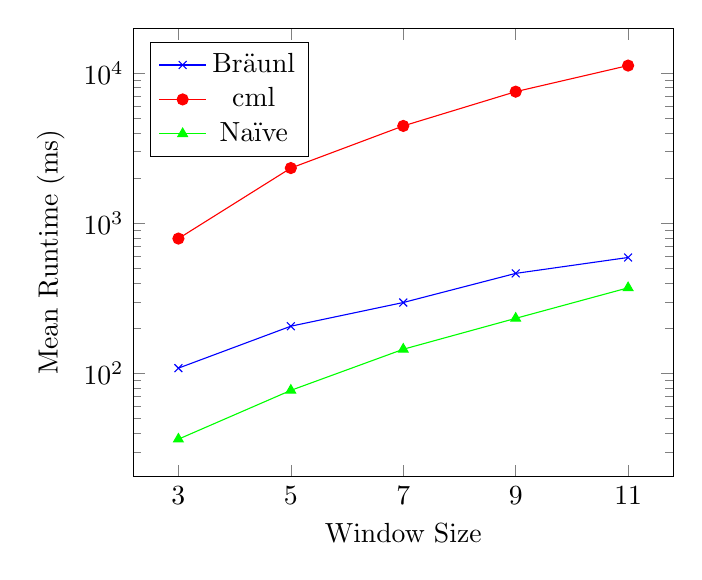
\begin{tikzpicture}
\begin{semilogyaxis}[
	xlabel=Window Size,
    ylabel=Mean Runtime (ms),
    legend pos=north west,
    %xmin=3,
    %xmax=11,
    %minor x tick num=2,
    xtick=data
]
	\addplot [mark=x,blue] table [x=windowSize,y=Mean]{
    	Method	windowSize	filename	Mean	Error	StdDev	Median	Min	Scaled	ScaledSD	Gen0	Gen1	Gen2	Allocated
Bräunl	3	peppers_gray	108.436	2.141	5.088	108.817	93.931	2.98	0.18	1200	1000	1000	37.73
Bräunl	5	peppers_gray	206.336	4.112	9.693	205.430	187.900	2.68	0.15	1000	666.6667	666.6667	58.64
Bräunl	7	peppers_gray	296.717	5.718	5.616	297.432	286.169	2.05	0.12	2000	1000	1000	114.81
Bräunl	9	peppers_gray	463.857	9.138	8.975	464.704	449.199	2	0.13	3000	2000	1000	127.86
Bräunl	11	peppers_gray	592.056	11.749	21.483	589.079	557.281	1.62	0.21	5000	2000	1000	212.34

    };
    \addplot [mark=*,red] table [x=windowSize,y=Mean]{
    	Method	windowSize	filename	Mean	Error	StdDev	Median	Min	Scaled	ScaledSD	Gen0	Gen1	Gen2	Allocated
\gls{cml}	3	peppers_gray	791.285	15.397	23.971	791.190	749.316	21.73	1.09	4000	2000	1000	28.14
\gls{cml}	5	peppers_gray	2333.317	46.639	79.197	2339.807	2108.572	30.29	1.42	8000	3000	2000	28.67
\gls{cml}	7	peppers_gray	4452.903	88.038	183.769	4407.427	4177.586	30.83	2.09	14000	5000	2000	28.28
\gls{cml}	9	peppers_gray	7533.048	150.341	225.023	7527.491	7100.467	32.49	2.2	21000	7000	2000	28.29
\gls{cml}	11	peppers_gray	11237.458	192.938	180.475	11266.773	10925.938	30.74	3.81	32000	10000	4000	29.38
    };
    \addplot [mark=triangle*,green] table [x=windowSize,y=Mean]{
    	Method	windowSize	filename	Mean	Error	StdDev	Median	Min	Scaled	ScaledSD	Gen0	Gen1	Gen2	Allocated
Naïve	3	peppers_gray	36.474	0.724	1.495	36.450	33.341	1	0	3357.1429	1000	1000	36.94
Naïve	5	peppers_gray	77.122	1.532	2.602	77.005	71.833	1	0	7285.7143	1000	1000	87.78
Naïve	7	peppers_gray	144.854	2.895	8.119	142.671	132.158	1	0	13750	1000	1000	175.21
Naïve	9	peppers_gray	232.750	5.198	15.245	227.335	213.438	1	0	21666.6667	1666.6667	1000	239.09
Naïve	11	peppers_gray	371.789	17.122	50.485	345.788	313.159	1	0	32000	1000	1000	337.86
    };
    
    \legend{Bräunl,\gls{cml},Naïve}
\end{semilogyaxis}
\end{tikzpicture}
\caption{\label{graph:median:peppers}Plot of mean runtimes with a logarithmic y axis for the peppers image}
\end{figure}

%small
\begin{figure}
\centering
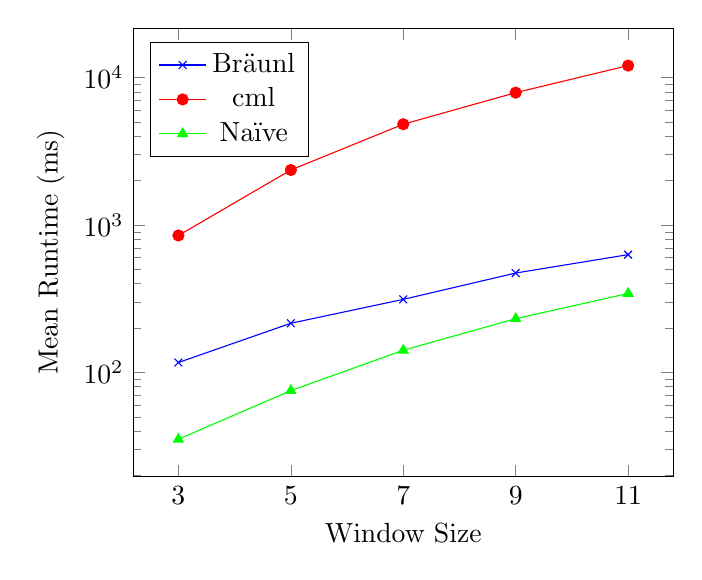
\begin{tikzpicture}
\begin{semilogyaxis}[
	xlabel=Window Size,
    ylabel=Mean Runtime (ms),
    legend pos=north west,
    %xmin=3,
    %xmax=11,
    %minor x tick num=2,
    xtick=data
]
	\addplot [mark=x,blue] table [x=windowSize,y=Mean]{
    	Method	windowSize	filename	Mean	Error	StdDev	Median	Min	Scaled	ScaledSD	Gen0	Gen1	Gen2	Allocated
Bräunl	3	small	116.782	2.334	4.208	116.874	107.437	3.32	0.14	1200	1000	800	40.96
Bräunl	5	small	215.573	4.295	12.185	217.475	180.880	2.86	0.16	1666.6667	1333.3333	1000	63.03
Bräunl	7	small	313.114	2.952	2.761	312.674	309.410	2.21	0.02	2000	1000	1000	111.37
Bräunl	9	small	472.517	4.680	4.378	473.456	460.456	2.04	0.02	4000	2000	1000	161.63
Bräunl	11	small	629.898	5.558	4.927	628.729	618.231	1.83	0.02	5000	2000	1000	149.05

    };
    \addplot [mark=*,red] table [x=windowSize,y=Mean]{
    	Method	windowSize	filename	Mean	Error	StdDev	Median	Min	Scaled	ScaledSD	Gen0	Gen1	Gen2	Allocated
\gls{cml}	3	small	849.482	19.570	56.149	828.209	773.390	24.12	1.69	4000	2000	1000	33.68
\gls{cml}	5	small	2362.643	46.461	104.871	2355.982	2162.910	31.39	1.39	9000	3000	2000	33.25
\gls{cml}	7	small	4830.294	95.856	137.474	4834.632	4523.971	34.15	0.97	14000	5000	2000	33.04
\gls{cml}	9	small	7910.925	134.530	125.839	7909.106	7701.102	34.15	0.54	23000	8000	3000	34.13
\gls{cml}	11	small	12074.170	232.388	228.236	12042.342	11712.425	35.17	0.66	32000	11000	3000	34

    };
    \addplot [mark=triangle*,green] table [x=windowSize,y=Mean]{
    	Method	windowSize	filename	Mean	Error	StdDev	Median	Min	Scaled	ScaledSD	Gen0	Gen1	Gen2	Allocated
Naïve	3	small	35.246	0.697	0.881	34.905	34.267	1	0	3466.6667	1000	1000	37.65
Naïve	5	small	75.282	0.506	0.473	75.217	74.419	1	0	7857.1429	1000	1000	95.36
Naïve	7	small	141.432	0.804	0.752	141.446	140.203	1	0	14000	1000	1000	175.74
Naïve	9	small	231.667	0.979	0.867	232.029	229.561	1	0	22666.6667	1666.6667	1000	328.08
Naïve	11	small	343.286	1.710	1.600	342.643	341.541	1	0	33000	1000	1000	261.29
    };
    
    \legend{Bräunl,\gls{cml},Naïve}
\end{semilogyaxis}
\end{tikzpicture}
\caption{\label{graph:median:small}Plot of mean runtimes with a logarithmic y axis for the small size image}
\end{figure}

%medium
\begin{figure}
\centering
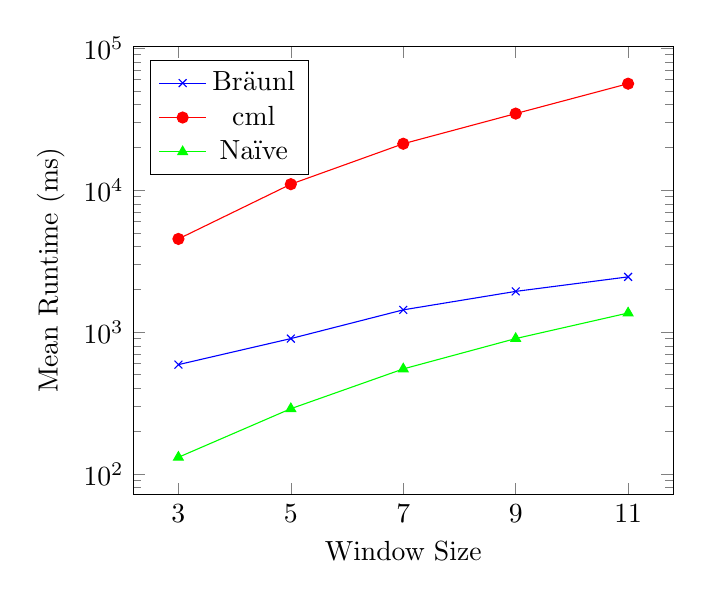
\begin{tikzpicture}
\begin{semilogyaxis}[
	xlabel=Window Size,
    ylabel=Mean Runtime (ms),
    legend pos=north west,
    %xmin=3,
    %xmax=11,
    %minor x tick num=2,
    xtick=data
]
	\addplot [mark=x,blue] table [x=windowSize,y=Mean]{
    	Method	windowSize	filename	Mean	Error	StdDev	Median	Min	Scaled	ScaledSD	Gen0	Gen1	Gen2	Allocated
Bräunl	3	medium	589.431	11.668	10.344	585.135	574.774	4.51	0.27	2000	1000	1000	146.49
Bräunl	5	medium	899.233	4.445	3.940	899.270	892.109	3.12	0.07	4000	2000	1000	230.3
Bräunl	7	medium	1433.220	31.164	29.151	1431.262	1379.761	2.61	0.07	7000	4000	2000	374.04
Bräunl	9	medium	1933.758	24.222	22.657	1925.642	1905.768	2.15	0.02	16000	4000	2000	527.35
Bräunl	11	medium	2447.284	47.271	50.580	2451.473	2352.536	1.8	0.05	40000	4000	2000	167.19

    };
    \addplot [mark=*,red] table [x=windowSize,y=Mean]{
    	Method	windowSize	filename	Mean	Error	StdDev	Median	Min	Scaled	ScaledSD	Gen0	Gen1	Gen2	Allocated
\gls{cml}	3	medium	4527.962	89.754	226.819	4511.961	4003.316	34.65	2.61	12000	6000	3000	132.41
\gls{cml}	5	medium	11006.775	197.445	184.691	10983.829	10737.131	38.19	1.05	28000	10000	4000	138.84
\gls{cml}	7	medium	21210.296	417.303	409.847	21118.240	20410.160	38.61	1.08	50000	15000	4000	136.78
\gls{cml}	9	medium	34587.347	471.655	441.186	34687.611	33898.247	38.45	0.48	81000	22000	4000	137.63
\gls{cml}	11	medium	56196.611	1118.853	2548.193	55158.372	52956.449	41.29	2.05	230000	66000	4000	132.75
    };
    \addplot [mark=triangle*,green] table [x=windowSize,y=Mean]{
    	Method	windowSize	filename	Mean	Error	StdDev	Median	Min	Scaled	ScaledSD	Gen0	Gen1	Gen2	Allocated
Naïve	3	medium	131.111	2.655	7.787	128.188	122.294	1	0	11500	1500	1500	102.34
Naïve	5	medium	288.343	5.716	6.805	285.656	282.623	1	0	28000	1000	1000	371.43
Naïve	7	medium	549.600	12.951	12.114	543.465	539.418	1	0	54000	1000	1000	710.4
Naïve	9	medium	899.563	3.131	2.444	900.523	893.992	1	0	89000	2000	1000	985.29
Naïve	11	medium	1361.629	27.108	31.217	1350.193	1344.088	1	0	131000	4000	1000	1969.78
    };
    
    \legend{Bräunl,\gls{cml},Naïve}
\end{semilogyaxis}
\end{tikzpicture}
\caption{\label{graph:median:medium}Plot of mean runtimes with a logarithmic y axis for the medium size image}
\end{figure}

%\gls{cml}
\begin{figure}
\centering
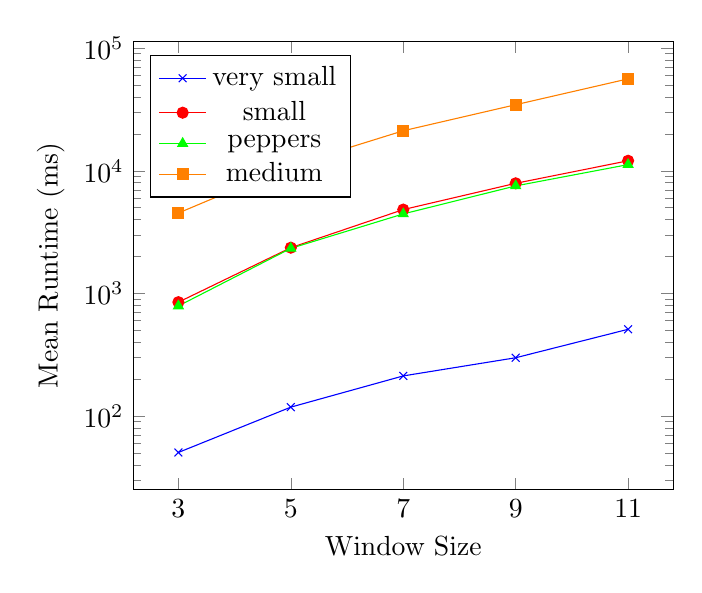
\begin{tikzpicture}
\begin{semilogyaxis}[
	xlabel=Window Size,
    ylabel=Mean Runtime (ms),
    legend pos=north west,
    %xmin=3,
    %xmax=11,
    %minor x tick num=2,
    xtick=data
]
	\addplot [mark=x,blue] table [x=windowSize,y=Mean]{
    	Method	windowSize	filename	Mean	Error	StdDev	Median	Min	Scaled	ScaledSD	Gen0	Gen1	Gen2	Allocated
\gls{cml}	3	very-small	50.588	2.544	7.500	49.480	40.127	31.18	4.6	166.6667	83.3333	-	1.68
\gls{cml}	5	very-small	118.463	2.349	3.443	119.399	106.345	29.75	0.99	400	200	-	1.69
\gls{cml}	7	very-small	212.817	7.252	21.270	220.862	152.973	28.08	2.79	1000	-	-	1.73
\gls{cml}	9	very-small	299.339	5.264	4.396	298.044	296.011	23.98	0.34	2000	1000	-	1.83
\gls{cml}	11	very-small	510.526	10.065	9.414	510.343	489.584	26.97	0.51	3000	1000	-	1.85


    };
    \addplot [mark=*,red] table [x=windowSize,y=Mean]{
    	Method	windowSize	filename	Mean	Error	StdDev	Median	Min	Scaled	ScaledSD	Gen0	Gen1	Gen2	Allocated
\gls{cml}	3	small	849.482	19.570	56.149	828.209	773.390	24.12	1.69	4000	2000	1000	33.68
\gls{cml}	5	small	2362.643	46.461	104.871	2355.982	2162.910	31.39	1.39	9000	3000	2000	33.25
\gls{cml}	7	small	4830.294	95.856	137.474	4834.632	4523.971	34.15	0.97	14000	5000	2000	33.04
\gls{cml}	9	small	7910.925	134.530	125.839	7909.106	7701.102	34.15	0.54	23000	8000	3000	34.13
\gls{cml}	11	small	12074.170	232.388	228.236	12042.342	11712.425	35.17	0.66	32000	11000	3000	34

    };
    \addplot [mark=triangle*,green] table [x=windowSize,y=Mean]{
    	Method	windowSize	filename	Mean	Error	StdDev	Median	Min	Scaled	ScaledSD	Gen0	Gen1	Gen2	Allocated
\gls{cml}	3	peppers_gray	791.285	15.397	23.971	791.190	749.316	21.73	1.09	4000	2000	1000	28.14
\gls{cml}	5	peppers_gray	2333.317	46.639	79.197	2339.807	2108.572	30.29	1.42	8000	3000	2000	28.67
\gls{cml}	7	peppers_gray	4452.903	88.038	183.769	4407.427	4177.586	30.83	2.09	14000	5000	2000	28.28
\gls{cml}	9	peppers_gray	7533.048	150.341	225.023	7527.491	7100.467	32.49	2.2	21000	7000	2000	28.29
\gls{cml}	11	peppers_gray	11237.458	192.938	180.475	11266.773	10925.938	30.74	3.81	32000	10000	4000	29.38
    };
    \addplot [mark=square*,orange] table [x=windowSize,y=Mean]{
    	Method	windowSize	filename	Mean	Error	StdDev	Median	Min	Scaled	ScaledSD	Gen0	Gen1	Gen2	Allocated
\gls{cml}	3	medium	4527.962	89.754	226.819	4511.961	4003.316	34.65	2.61	12000	6000	3000	132.41
\gls{cml}	5	medium	11006.775	197.445	184.691	10983.829	10737.131	38.19	1.05	28000	10000	4000	138.84
\gls{cml}	7	medium	21210.296	417.303	409.847	21118.240	20410.160	38.61	1.08	50000	15000	4000	136.78
\gls{cml}	9	medium	34587.347	471.655	441.186	34687.611	33898.247	38.45	0.48	81000	22000	4000	137.63
\gls{cml}	11	medium	56196.611	1118.853	2548.193	55158.372	52956.449	41.29	2.05	230000	66000	4000	132.75
    };
    
    \legend{very small,small,peppers,medium}
\end{semilogyaxis}
\end{tikzpicture}
\caption[Plot of mean runtimes for the \glsentrylong{cml-glossary} algorithm on different image sizes]{\label{graph:median:cmls}Plot of mean runtimes with a logarithmic y axis for the \gls{cml} algorithm on different image sizes}
\end{figure}

\begin{figure}
\centering
\subcaptionbox{Original}{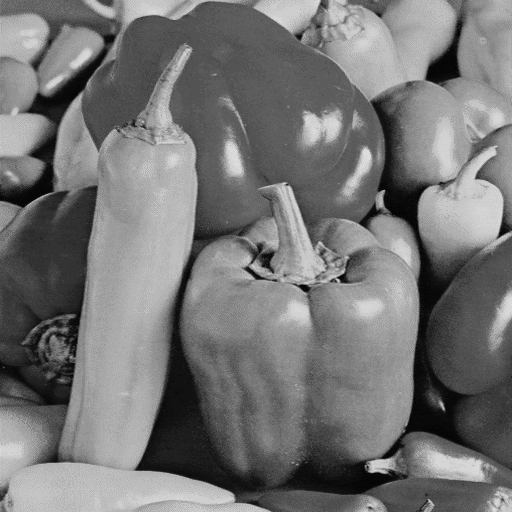
\includegraphics[width=0.41\textwidth]{chapters/medianfilter/images/peppers/peppers_gray.png}}
\subcaptionbox{Noisy}{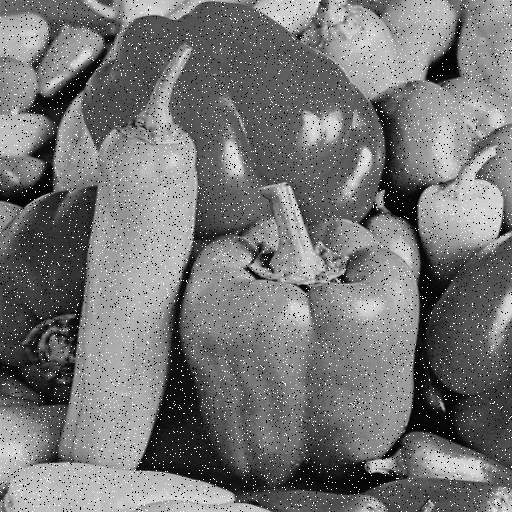
\includegraphics[width=0.41\textwidth]{chapters/medianfilter/images/peppers/peppers_gray_noisy.png}}
\subcaptionbox{Naïve}{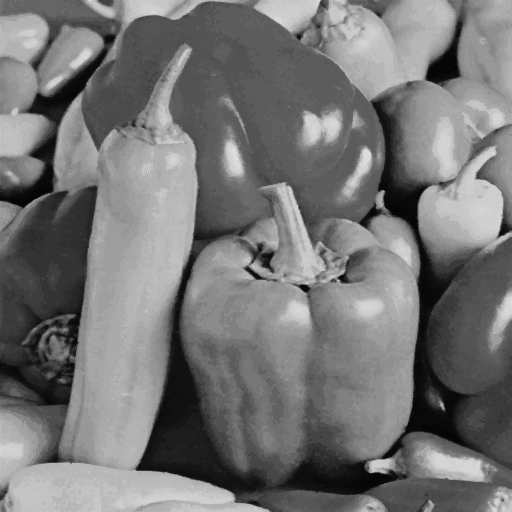
\includegraphics[width=0.41\textwidth]{chapters/medianfilter/images/peppers/naive_peppers_gray_noisy_3.png}}
\subcaptionbox{Bräunl}{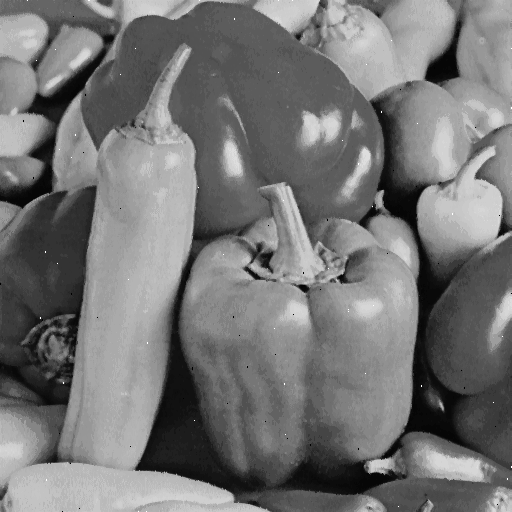
\includegraphics[width=0.41\textwidth]{chapters/medianfilter/images/peppers/braunl_peppers_gray_noisy_3.png}}
\subcaptionbox{\gls{cml}}{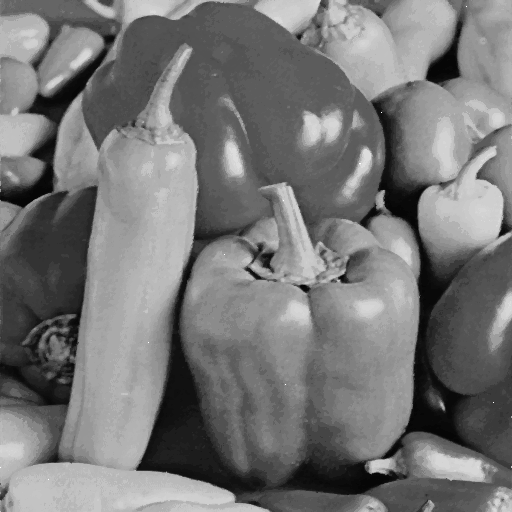
\includegraphics[width=0.41\textwidth]{chapters/medianfilter/images/peppers/cml_peppers_gray_noisy_3.png}}
\caption[The classic grayscale `peppers' image, before and after processing]{\label{fig:median:peppers}The classic greyscale `peppers' image, before and after processing.  (a) is the original image; (b) is the image with random salt \& pepper noise introduced; (c) is the result of processing the image using the naïve algorithm; (d) is the result of processing the image using the Br\"{a}unl-inspired algorithm; (e) is the result of processing the image using the \gls{cml} algorithm}
\end{figure}

\begin{table}
\centering
\caption[Peak signal-to-noise for the very small image]{Peak signal-to-noise ratio for the very small image (measured in decibels)}
\label{tab:median:psnrvsmall}
\begin{tabular}{@{}lccccc@{}}
\toprule
\multicolumn{1}{c}{\textbf{Algorithm}} & \multicolumn{5}{c}{\textbf{Window size}}                                          \\
                                       & 3              & 5              & 7              & 9             & 11             \\ \midrule
Bräunl                                 & 20.78          & 17.82          & 15.65          & 14.36         & 13.55          \\
\gls{cml}                                    & 25.98          & \textbf{21.85} & \textbf{18.62} & \textbf{16.40} & 14.99          \\
Naïve                                  & \textbf{27.03} & 21.74          & 18.55          & 16.39         & \textbf{15.02} \\ \bottomrule
\end{tabular}
\end{table}

\begin{table}
\centering
\caption[Peak signal-to-noise for the peppers image]{Peak signal-to-noise ratio for the peppers image (measured in decibels)}
\begin{tabular}{@{}lccccc@{}}
\toprule
\multicolumn{1}{c}{\textbf{Algorithm}} & \multicolumn{5}{c}{\textbf{Window size}}                                          \\
                                       & 3              & 5              & 7              & 9              & 11            \\ \midrule
Bräunl                                 & 28.76          & 27.35          & 25.27          & 23.94          & 22.82         \\
\gls{cml}                                    & 31.85          & 31.07          & 29.8           & 28.56          & 27.42         \\
Naïve                                  & \textbf{32.79} & \textbf{31.25} & \textbf{29.87} & \textbf{28.63} & \textbf{27.50} \\ \bottomrule
\end{tabular}
\label{tab:median:psnrpeppers}
\end{table}

\begin{table}
\centering
\caption[Peak signal-to-noise for the small image]{Peak signal-to-noise ratio for the small image (measured in decibels)}
\label{tab:median:psnrsmall}
\begin{tabular}{@{}lccccc@{}}
\toprule
\multicolumn{1}{c}{\textbf{Algorithm}} & \multicolumn{5}{c}{\textbf{Window size}}                                          \\
                                       & 3              & 5              & 7             & 9              & 11             \\ \midrule
Bräunl                                 & 32.83          & 32.34          & 30.74         & 29.73          & 28.94          \\
\gls{cml}                                    & 36.62          & 34.25          & 32.66         & 31.57          & 30.71          \\
Naïve                                  & \textbf{37.83} & \textbf{34.31} & \textbf{32.7} & \textbf{31.65} & \textbf{30.81} \\ \bottomrule
\end{tabular}
\end{table}

\begin{table}
\centering
\caption[Peak signal-to-noise for the medium image]{Peak signal-to-noise ratio for the medium image (measured in decibels)}
\begin{tabular}{@{}lccccc@{}}
\toprule
\multicolumn{1}{c}{\textbf{Algorithm}} & \multicolumn{5}{c}{\textbf{Window size}}                                           \\
                                       & 3              & 5              & 7              & 9              & 11             \\ \midrule
Bräunl                                 & 32.98          & 32.65          & 31.59          & 30.91          & 30.36          \\
\gls{cml}                                    & 36.72          & \textbf{34.15} & \textbf{32.98} & \textbf{32.26} & \textbf{31.73} \\
Naïve                                  & \textbf{37.16} & 34.07          & 32.96          & \textbf{32.26} & \textbf{31.73} \\ \bottomrule
\end{tabular}
\label{tab:median:psnrmedium}
\end{table}

Examination of the reported memory statistics (please see the GitHub repository for details) appears to show that the maximum amount of memory allocated during processing for the \gls{cml} algorithm stays roughly constant across window sizes for each image size, and in fact on larger window sizes it is the most memory efficient.  The naïve algorithm quickly grows to consume the most memory at larger window sizes for each image size, suggesting that it likely derives some of its comparative speed at the cost of greater space complexity, while Bräunl sits in the middle.  Conversely, \gls{cml} generates by far the most garbage collection events, which may help explain its relative sluggishness.

\section{Discussion}

The algorithms developed and presented here are not necessarily optimal for the purpose.  They largely handle each pixel separately, or combine them into arrays on-the-fly.  This ignores the possibility of exploiting data-parallelism to improve throughput, and instead relies only on the separate CPU cores to provide parallelism.

It is unclear how much the mechanics underlying these implementations (\ie{} the .NET Core and \hopac{} systems) attempt to maximise use of the processor cache.  Efficient use of the cache can contribute significantly to an optimised version of an algorithm outperforming, a simplistic version by an order of magnitude or more \cite{Ragan-Kelley2017}.  No attempt was made manually to ensure good practices, such as tiling or striping \cite{Midkiff2012}.

The \gls{cml} approach used in essence instantiates a \gls{pe} for each pixel, each of which must be scheduled to run at some point --- concurrent with another \gls{pe} in the case of synchronous message passing.  It is possible that this surfeit of separate logical threads may induce excessive switching costs, and perhaps promote wasted time, with threads regularly polling their channel and their neighbours'.  Careful improvements to this and the use of the cache might lead to significant gains in speed.

In terms of the code itself also, \gls{cml} appears to be the worst.  The program requires roughly double the number of lines of the naïve program, and is arguably much less `clean' or `readable'.  Reinterpreting the \gls{medianfilter} in terms of \glsxtrlong{csp} has not yielded a structural improvement nor simplified the programming task.  Combined with the running time results above, this suggests that the \gls{cml} approach is actively counter-productive for implementing \glspl{mwt}, at least when using \hopac{}.

Basic profiling of the \gls{cml}-based implementation appears to show that more than half of the runtime of the program was spent inside the function for giving a value over a channel, and functions called by it.  Furthermore, according to this profiling, almost 40\% of the total running time of the algorithm is taken up specifically by low-level memory management functions inside the depths of the .NET Core system.  Considering that some of these functions \fxwarning{ref?}{are written in hand-optimised assembly}, the fact they account for so much of the running time appears to suggest that memory use is poorly handled in the tested implementation.

\Glspl{mwt} are generally relatively simplistic processes, typically consisting simply of combining values from the pixel array, and which can be programmed in a straightforward fashion.  More sophisticated programming techniques may simply `get in the way' and introduce unnecessary overheads, which appears to have happened here.  Furthermore, the \gls{medianfilter} can largely be broken down into arithmetic and logical operations amenable to vectorisation (\eg{} \cite{Sanchez2012,Perreault2007}), which the \gls{cml} approach currently ignores entirely.

% \subsection{Threats to validity}
\subsection{Experimental Limitations}
There are two identifiable threats to validity, both regarding the `quality' of the programming involved.  .NET Core, as a widely used open-source compiler and runtime system, and which has likely had millions of man-hours invested in it, is presumably of high quality and fast in most cases.  That is not necessarily the case with \hopac{}.  While it is open source, and moderately well-known in the \fsharp{} community, the amount of time spent on optimising it is likely nowhere close to that spent on .NET Core.  Consequently, \hopac{} itself may present significant bottlenecks while performing the \gls{mwt}.

The other threat to validity (as with all performance-focused experiments) is the skill of the end programmer.  The author was new to the \hopac{} library at the start of this work, and inferior design choices may have been made unwittingly.  It was, however, suggested during personal communication with one of the maintainers and fellow users of the \hopac{} library that the \gls{cml} approach may simply be a poor fit to pixel-wise image processing tasks.

Fundamentally, the results achieved here, as with most implementation exercises, succeed or fail in large part on the skill, knowledge and effort of the programmers involved.  The use of other libraries may lead to better results.  Other parallel implementations of \gls{cml} exist, such as Concurrent Haskell \cite{Chaudhuri2009}, Manticore \cite{Reppy2009a} and Fibers\footnote{\url{https://github.com/wingo/fibers}} for Guile Scheme, but have not been assessed for this work.